%%%%%%%%%%%%%%%%%%%%%%%%%%%%%%%%%%%%
% Slide options
%%%%%%%%%%%%%%%%%%%%%%%%%%%%%%%%%%%%

% Option 1: Slides with solutions

\documentclass[slidestop,compress,mathserif]{beamer}
\usepackage{booktabs}
\newcommand{\soln}[1]{\textit{#1}}
\newcommand{\solnGr}[1]{#1}

% Option 2: Handouts without solutions

%\documentclass[11pt,containsverbatim,handout]{beamer}
%\usepackage{pgfpages}
%\pgfpagesuselayout{4 on 1}[letterpaper,landscape,border shrink=5mm]
%\newcommand{\soln}[1]{ }
%\newcommand{\solnGr}{ }

%%%%%%%%%%%%%%%%%%%%%%%%%%%%%%%%%%%%
% Style
%%%%%%%%%%%%%%%%%%%%%%%%%%%%%%%%%%%%
%%%%%%%%%%%%%%%%%%%%%%%%%%%%%%%%%%%%%%%%%%%%%%%%%%%%%%%%%%%%%%%%%%%%%%%%
% MA213/214 shared slide style
%
% "Calm & Cool" palette + content-type callout boxes.
% Overhauled (2026) from the original OpenIntro/metropolis style:
%   - all OpenIntro visual branding removed (logo, grid, colors)
%   - a low-key cool palette (see colors below)
%   - tcolorbox callout boxes so students recognize content types
% See common/README.md for the command cheat-sheet.
%%%%%%%%%%%%%%%%%%%%%%%%%%%%%%%%%%%%%%%%%%%%%%%%%%%%%%%%%%%%%%%%%%%%%%%%

\usetheme{metropolis}

%%%%%%%%%%%%%%%%
% Packages
%%%%%%%%%%%%%%%%

\usepackage{geometry}
\usepackage{graphicx}
\usepackage{amssymb}
\usepackage{epstopdf}
\usepackage{amsmath}  	% this permits text in eqnarray among other benefits
\usepackage{url}		% produces hyperlinks
\usepackage{hyperref}	% allows for color usage in tables
\usepackage[english]{babel}
\usepackage[latin1]{inputenc}
\usepackage{colortbl}	% allows for color usage in tables
\usepackage{multirow}	% allows for rows that span multiple rows in tables
\usepackage{color}		% this package has a variety of color options
\usepackage{pgf}
\usepackage{calc}
\usepackage{ulem}
\usepackage{multicol}
\usepackage{textcomp}
\usepackage{txfonts}
\usepackage{listings}
\usepackage{tikz}
\usepackage{array}
\usepackage{wasysym}
\usepackage{fancyvrb}
\usepackage{etoolbox}             % \ifstrempty for optional box subtitles
\usepackage[most]{tcolorbox}      % content-type callout boxes
\tcbuselibrary{listings}          % R-code block (\begin{rblock})
\usepackage{fontawesome5}         % box icons

%%%%%%%%%%%%%%%%
% Remove navigation symbols
%%%%%%%%%%%%%%%%

\setbeamertemplate{navigation symbols}{}

%%%%%%%%%%%%%%%%
% "Calm & Cool" palette
%%%%%%%%%%%%%%%%

% chrome / structure / body
\definecolor{ccSlate}{HTML}{2E3742}   % frametitle bar, structure, section pages (deep neutral slate)
\definecolor{ccInk}{HTML}{2B2B2B}     % body text
\definecolor{ccWash}{HTML}{FCF8F1}    % gentle warm title-slide background wash (complements the cool blues)

% example (blue)
\definecolor{ccBlue}{HTML}{2F6690}
\definecolor{ccBlueBg}{HTML}{EAF1F7}
% interactive activity / discussion (green)
\definecolor{ccGreen}{HTML}{4E8A6B}
\definecolor{ccGreenBg}{HTML}{E9F3EC}
% solution (purple)
\definecolor{ccPurple}{HTML}{6F5499}
\definecolor{ccPurpleBg}{HTML}{EFEAF6}
% worksheet / focused work (terracotta)
\definecolor{ccTerra}{HTML}{C2693E}
\definecolor{ccTerraBg}{HTML}{FAEDE4}
% formula / definition (neutral slate)
\definecolor{ccGray}{HTML}{5C6B7A}
\definecolor{ccGrayBg}{HTML}{EEF1F4}
% caution / common pitfall (brick red)
\definecolor{ccRed}{HTML}{B23A48}
\definecolor{ccRedBg}{HTML}{FAEAEC}
% key idea / takeaway (muted gold)
\definecolor{ccGold}{HTML}{9C7A28}
\definecolor{ccGoldBg}{HTML}{F7F1DF}
% learning goals / lesson outcomes (teal)
\definecolor{ccTeal}{HTML}{2C6E6B}
\definecolor{ccTealBg}{HTML}{E6F0EF}
% learning objectives (indigo)
\definecolor{ccIndigo}{HTML}{45507A}
\definecolor{ccIndigoBg}{HTML}{ECEEF4}
% R code / output (gray)
\definecolor{ccCode}{HTML}{5F5E5A}
\definecolor{ccCodeBg}{HTML}{F4F5F6}

% neutral grays kept from the original style
\definecolor{gray}{rgb}{0.5, 0.5, 0.5}
\definecolor{darkGray}{rgb}{0.3, 0.3, 0.3}
\definecolor{darkerGray}{rgb}{0.2, 0.2, 0.2}

% Backwards-compatible aliases: old OpenIntro color names now point at the
% new palette, so existing \textcolor{oiB}{...}, \hl{...}, etc. keep working.
\colorlet{oiB}{ccBlue}
\colorlet{oiG}{ccGreen}
\colorlet{hlblue}{ccBlue}
\colorlet{rubineRed}{ccRed}
\colorlet{irishGreen}{ccGreen}
\colorlet{lightGreen}{ccGreen}

%%%%%%%%%%%%%%%%
% Restyle metropolis with the Calm & Cool chrome
%%%%%%%%%%%%%%%%

\metroset{block=fill}

\setbeamercolor{normal text}{fg=ccInk, bg=white}
\setbeamercolor{structure}{fg=ccSlate}
\setbeamercolor{alerted text}{fg=ccBlue}
\setbeamercolor{example text}{fg=ccGreen}
\setbeamercolor{frametitle}{bg=ccSlate, fg=white}
\setbeamercolor{progress bar}{fg=ccBlue}
\setbeamercolor{title separator}{fg=ccBlue}
\setbeamercolor{title}{fg=ccSlate}
\setbeamercolor{subtitle}{fg=ccBlue}
\setbeamercolor{author}{fg=ccInk}
\setbeamercolor{institute}{fg=ccGray}
\setbeamercolor{date}{fg=ccGray}
\setbeamercolor{section title}{fg=ccSlate}
\setbeamercolor{standout}{fg=white, bg=ccSlate}

% Section pages sit on the same warm wash as the title slide. We keep
% metropolis's section-title styling and just paint a full-page ccWash
% background behind it (needs >=2 pdflatex passes for the current-page node).
\setbeamertemplate{section page}{%
  \begin{tikzpicture}[remember picture, overlay]
    \fill[ccWash] (current page.south west) rectangle (current page.north east);
  \end{tikzpicture}%
  \centering
  \begin{minipage}{22em}
    \raggedright
    \usebeamercolor[fg]{section title}%
    \usebeamerfont{section title}%
    \insertsectionhead\\[-1ex]
    \usebeamertemplate*{progress bar in section page}%
    \par
  \end{minipage}\par
  \vspace{\baselineskip}
}

%%%%%%%%%%%%%%%%
% Custom inline text commands (recolored to the palette)
%%%%%%%%%%%%%%%%

% degree
\newcommand{\degree}{\ensuremath{^\circ}}

% cite
\newcommand{\ct}[1]{
\vfill
{\tiny #1}}

\newcommand{\NamedNote}[2]{
\rule{2.5cm}{0.25pt} \\ \textit{\footnotesize{\textcolor{rubineRed}{#1:} \textcolor{darkerGray}{#2}}}}

% Note
\newcommand{\Note}[1]{
\rule{2.5cm}{0.25pt} \\ \textit{\footnotesize{\textcolor{rubineRed}{Note:} \textcolor{darkerGray}{#1}}}}

% Remember
\newcommand{\Remember}[1]{\textit{\scriptsize{\textcolor{ccTerra}{Remember:} #1}}}

% expected counts
\newcommand{\ex}[1]{\textit{\textcolor{ccBlue}{#1}}}

% red
\newcommand{\red}[1]{\textit{\textcolor{rubineRed}{#1}}}

% pink
\newcommand{\pink}[1]{\textit{\textcolor{rubineRed!90!white!50}{#1}}}

% green
\newcommand{\green}[1]{\textit{\textcolor{irishGreen}{#1}}}

% orange
\newcommand{\orange}[1]{\textit{\textcolor{ccTerra}{#1}}}

% links: webURL, webLink, appLink
\newcommand{\webURL}[1]{\urlstyle{same}{ \textit{\textcolor{darkGray}{\url{#1}}}}}
\newcommand{\webLink}[2]{\href{#1}{\textcolor{darkGray}{{#2}}}}
\newcommand{\appLink}[2]{\href{#1}{\textcolor{white}{{#2}}}}

% mail
\newcommand{\mail}[1]{\href{mailto:#1}{\textit{\textcolor{darkGray}{#1}}}}

% highlighting: hl, hlGr, mathhl
\newcommand{\hl}[1]{\textit{\textcolor{hlblue}{#1}}}
\newcommand{\hlGr}[1]{\textit{\textcolor{lightGreen}{#1}}}
\newcommand{\mathhl}[1]{\textcolor{hlblue}{\ensuremath{#1}}}

%%%%%%%%%%%%%%%%
% Structural helpers (unchanged from the original)
%%%%%%%%%%%%%%%%

% two col: two columns
\newenvironment{twocol}[4]{
\begin{columns}[c]
\column{#1\textwidth}
#3
\column{#2\textwidth}
#4
\end{columns}
}

% slot (for probability calculations)
\newenvironment{slot}[2]{
\begin{array}{c}
\underline{#1} \\
#2
\end{array}
}

% pr: left and right parentheses
\newcommand{\pr}[1]{
\left( #1 \right)
}

% cancel
\newcommand{\cancel}[1]{%
    \tikz[baseline=(tocancel.base)]{
        \node[inner sep=0pt,outer sep=0pt] (tocancel) {#1};
        \draw[red, line width=0.5mm] (tocancel.south west) -- (tocancel.north east);
    }%
}

% removepagenumbers
\newcommand{\removepagenumbers}{%
  \setbeamertemplate{footline}{}
}

% change margin
\newenvironment{changemargin}[2]{%
\begin{list}{}{%
\setlength{\topsep}{0pt}%
\setlength{\leftmargin}{#1}%
\setlength{\rightmargin}{#2}%
\setlength{\listparindent}{\parindent}%
\setlength{\itemindent}{\parindent}%
\setlength{\parsep}{\parskip}%
}%
\item}{\end{list}}

% footnote
\long\def\symbolfootnote[#1]#2{\begingroup%
\def\thefootnote{\fnsymbol{footnote}}\footnote[#1]{#2}\endgroup}

% commands from the book
\newenvironment{data}[1]{\texttt{#1}}{}
\newenvironment{var}[1]{\texttt{#1}}{}
\newenvironment{resp}[1]{\texttt{#1}}{}

%%%%%%%%%%%%%%%%
% Content-type callout boxes (tcolorbox)
%
% Each type has a colored title strip (icon + label) over a light fill.
% Color = content type; the label + icon reinforce it (so the cue does
% not rely on color alone).
%%%%%%%%%%%%%%%%

\tcbset{
  cccallout/.style 2 args={
    enhanced, breakable=false,
    colback=#2, colframe=#1, colbacktitle=#1, coltitle=white,
    fonttitle=\bfseries\footnotesize,
    boxrule=0.6pt, arc=2.5pt, outer arc=2.5pt,
    left=5pt, right=5pt, top=3pt, bottom=3pt, boxsep=2pt,
    toptitle=2pt, bottomtitle=2pt, lefttitle=5pt,
    before skip=5pt, after skip=5pt,
  },
}

% One-off / collection of examples (blue): \workedexample[subtitle]{body}.
% (Named \workedexample, not \example, because beamer defines \example.)
\newtcolorbox{examplebox}[1][]{cccallout={ccBlue}{ccBlueBg},
  title={\faIcon{lightbulb}~~Example\ifstrempty{#1}{}{ \textmd{---}\ #1}}}
\newcommand{\workedexample}[2][]{\begin{examplebox}[#1]#2\end{examplebox}}

% Running-example header (blue): \examplehead{name} at the top of each frame of a
% multi-slide running example. A one-off or a collection of examples uses the
% \workedexample box above instead.
\newcommand{\examplehead}[1]{%
  \vspace{-0.4em}\par\noindent\tcbox[on line, colback=ccBlue, colframe=ccBlue, coltext=white,
    boxrule=0pt, arc=2pt, left=5pt, right=5pt, top=1pt, bottom=1pt,
    box align=base, nobeforeafter]{\footnotesize\bfseries\faIcon{lightbulb}\,Running example}%
  \ifstrempty{#1}{}{\enspace{\footnotesize\bfseries\textcolor{ccBlue}{#1}}}%
  \par\nobreak\vspace{-0.6em}{\color{ccBlue}\rule{\linewidth}{0.7pt}}\par\nobreak\vspace{-0.8em}}

% Interactive activity (green): \activity[subtitle]{body}
\newtcolorbox{activitybox}[1][]{cccallout={ccGreen}{ccGreenBg},
  title={\faIcon{users}~~Activity\ifstrempty{#1}{}{ #1}}}
\newcommand{\activity}[2][]{\begin{activitybox}[#1]#2\end{activitybox}}

% Discussion question (green): \dq{body}
\newtcolorbox{dqbox}{cccallout={ccGreen}{ccGreenBg}, title={\faIcon{comments}~~Discussion}}
\newcommand{\dq}[1]{\begin{dqbox}#1\end{dqbox}}

% Solution (purple): \solnbox{body}. Gated by the per-deck \soln toggle, so it
% shows in the instructor build and vanishes from the student handout build.
% (Named \solnbox, not \solution, because beamer already defines \solution.)
\newtcolorbox{solutionbox}{cccallout={ccPurple}{ccPurpleBg}, title={\faIcon{key}~~Solution}}
\newcommand{\solnbox}[1]{\soln{\begin{solutionbox}#1\end{solutionbox}}}

% Worksheet / focused work (terracotta): \worksheet[subtitle]{body}
\newtcolorbox{worksheetbox}[1][]{cccallout={ccTerra}{ccTerraBg},
  title={\faIcon{pencil-alt}~~Worksheet\ifstrempty{#1}{}{ #1}}}
\newcommand{\worksheet}[2][]{\begin{worksheetbox}[#1]#2\end{worksheetbox}}

% Formula / definition (neutral slate). Supports both real usages found in the
% decks: \formula{title}{body} and the bare \formula{body} (title defaults to
% "Formula"). The second group is an optional brace argument.
\newtcolorbox{formulabox}[1][Formula]{cccallout={ccGray}{ccGrayBg},
  title={\faIcon{square-root-alt}~~#1}}
\NewDocumentCommand{\formula}{m g}{%
  \IfNoValueTF{#2}%
    {\begin{formulabox}#1\end{formulabox}}%
    {\begin{formulabox}[#1]#2\end{formulabox}}}

% Common pitfall / caution (brick red): \caution[subtitle]{body}
\newtcolorbox{cautionbox}[1][]{cccallout={ccRed}{ccRedBg},
  title={\faIcon{exclamation-triangle}~~Caution\ifstrempty{#1}{}{ #1}}}
\newcommand{\caution}[2][]{\begin{cautionbox}[#1]#2\end{cautionbox}}

% Key idea / takeaway (muted gold): \keyidea[subtitle]{body}
\newtcolorbox{keyideabox}[1][]{cccallout={ccGold}{ccGoldBg},
  title={\faIcon{star}~~Key idea\ifstrempty{#1}{}{ #1}}}
\newcommand{\keyidea}[2][]{\begin{keyideabox}[#1]#2\end{keyideabox}}

% Learning goals / lesson outcomes (teal): \goals{body}. Sits under the short
% LO headings on the objectives slide; body is the "you should be able to" list.
\newtcolorbox{goalsbox}{cccallout={ccTeal}{ccTealBg}, fontupper=\footnotesize,
  top=1pt, bottom=2pt, boxsep=1pt, before skip=3pt,
  title={\faIcon{bullseye}~~By the end of today, you should be able to\ldots}}
\newcommand{\goals}[1]{\begin{goalsbox}#1\end{goalsbox}}

% Learning objectives (indigo): \objectives{body} -- the formal LO headings,
% shown alongside \goals on the objectives slide.
\newtcolorbox{objectivesbox}{cccallout={ccIndigo}{ccIndigoBg}, fontupper=\small,
  top=1pt, bottom=2pt, boxsep=1pt, before skip=3pt,
  title={\faIcon{clipboard-list}~~Learning objectives}}
\newcommand{\objectives}[1]{\begin{objectivesbox}#1\end{objectivesbox}}

% Defaults for a bare \begin{lstlisting}. Without these it inherits the listings
% package defaults: 11pt type, fixed-width columns (which spaces code out as
% "a g e _ f i t"), and no line breaking, so a long line silently runs off the
% right edge of the slide. A deck that passes its own basicstyle still wins.
% Layout only -- syntax coloring is left to the \begin{rblock} environment.
\lstset{
  basicstyle=\ttfamily\footnotesize, columns=fullflexible,
  breaklines=true, breakindent=1.5em, showstringspaces=false,
  numbers=none, frame=none}

% R code / output (gray): \begin{rblock}[subtitle] ... \end{rblock}
% NOTE: a frame containing an rblock must be declared \begin{frame}[fragile].
\lstdefinestyle{ccR}{
  language=R, basicstyle=\ttfamily\footnotesize, columns=fullflexible,
  breaklines=true, showstringspaces=false, numbers=none, frame=none,
  keywordstyle=\color{ccBlue}, commentstyle=\color{ccGreen!75!black},
  stringstyle=\color{ccTerra}}
\newtcblisting{rblock}[1][]{cccallout={ccCode}{ccCodeBg},
  title={\faIcon{terminal}~~R\ifstrempty{#1}{}{ #1}},
  listing only, listing style=ccR}

% --- Legacy boxes (kept so existing decks compile) ---

% app: application exercise -> alias of activity
\newcommand{\app}[1]{\activity{#1}}

% pq: practice question (green, interactive family)
\newtcolorbox{pqbox}{cccallout={ccGreen}{ccGreenBg}, title={\faIcon{list-ol}~~Practice}}
\newcommand{\pq}[1]{\begin{pqbox}#1\end{pqbox}}

% solnMult: solutions for multiple-choice practice questions (uses \soln toggle)
\newcommand{\solnMult}[1]{
\item[] \vspace{-0.59cm}
\only<1>{\item #1}
\soln{\only<2->{\item \orange{#1}}}
}

%%%%%%%%%%%%%%%%
% De-branded title frame + attribution
%%%%%%%%%%%%%%%%

% Eyebrow line on the title slide; a deck may \renewcommand this.
\newcommand{\coursetag}{MA214: Applied Statistics}

% Attribution: all slides released under CC BY-SA, crediting both the
% instructor (later material) and OpenIntro (basis of the earlier material).
\newcommand{\courseattribution}{%
  Slides by Jonathan H.~Huggins, building on materials from OpenIntro's
  \emph{Introduction to Modern Statistics} (Mine \c{C}etinkaya-Rundel et al.).
  Released under the
  \webLink{http://creativecommons.org/licenses/by-sa/3.0/us/}{CC BY-SA license}.
  Some images included under fair use (educational purposes).}

% \maketitleframe: de-branded title slide (no logo, no grid). Uses the deck's
% \title, \subtitle, and \coursetag.
\newcommand{\maketitleframe}{%
  \addtocounter{framenumber}{-1}%
  {\removepagenumbers
  \setbeamercolor{background canvas}{bg=ccWash}%
  \begin{frame}[plain]
    \vspace*{2.6em}
    {\color{ccSlate}\rule{\textwidth}{2.5pt}}\par\vspace{1.5em}
    {\usebeamerfont{date}\scshape\color{ccGray}\coursetag}\par\vspace{0.55em}
    {\usebeamerfont{title}\color{ccSlate}\inserttitle\par}
    \vspace{0.45em}{\color{ccBlue}\rule{3em}{2.5pt}}\par\vspace{0.7em}
    {\usebeamerfont{subtitle}\color{ccBlue}\insertsubtitle\par}
    \vfill
    {\color{ccGray!55}\rule{\textwidth}{0.4pt}}\par\vspace{0.45em}
    {\tiny\color{ccGray}\courseattribution\par}
    \vspace*{0.4em}
  \end{frame}}}

%%%%%%%%%%%%%%%%
% Graphics
%%%%%%%%%%%%%%%%

\DeclareGraphicsRule{.tif}{png}{.png}{`convert #1 `dirname #1`/`basename #1 .tif`.png}

% The "why do they keep coming out bell-shaped?" slide shows the Lecture 8 and
% Lecture 9 figures side by side. Read them from those lectures' own figures/
% directories, where their R scripts write them, rather than keeping copies
% here that would silently fall out of date.
\graphicspath{ {../../common/} {figures/} {../lecture08/figures/} {../lecture09/figures/} }


%%%%%%%%%%%%%%%%%%%%%%%%%%%%%%%%%%%%
% Preamble
%%%%%%%%%%%%%%%%%%%%%%%%%%%%%%%%%%%%

\title[Lecture 10]{Lecture 10: Inference with mathematical models}
\subtitle{Module 2: Statistical Inference}
\author{Introduction to Modern Statistics, 2nd Edition}
\institute{$\:$ \\ {\footnotesize Based on slides developed by Mine \c{C}etinkaya-Rundel of OpenIntro.  \\
The slides may be copied, edited, and/or shared via the \webLink{http://creativecommons.org/licenses/by-sa/3.0/us/}{CC BY-SA license.} \\
Some images may be included under fair use guidelines (educational purposes).}}
\date{}

%%%%%%%%%%%%%%%%%%%%%%%%%%%%%%%%%%%%
% Begin document
%%%%%%%%%%%%%%%%%%%%%%%%%%%%%%%%%%%%

\begin{document}


%%%%%%%%%%%%%%%%%%%%%%%%%%%%%%%%%%%%
% Title page
%%%%%%%%%%%%%%%%%%%%%%%%%%%%%%%%%%%%

\maketitleframe

% !TEX root =  Lecture11.tex


%%%%%%%%%%%%%%%%%%%%%%%%%%%%%%%%%%%%
% Recap/Agenda
%%%%%%%%%%%%%%%%%%%%%%%%%%%%%%%%%%%%
\begin{frame}
\frametitle{Module 2: Statistical Inference}
    \begin{itemize}
        \item \hl{Previously:} confidence intervals by \emph{bootstrapping} --- resample the data, then read the interval off the simulated distribution.
        \item \hl{This time:} the same intervals and p-values, from \emph{formulas}.
          \begin{itemize}
              \item exact calculations: the binomial and the normal model;
              \item the central limit theorem --- and why our simulated distributions kept coming out bell-shaped;
              \item p-values and confidence intervals with $z$ and $t$;
              \item two-sample and paired data.
          \end{itemize}
        \item \hl{Reading:} IMS Chapter 13.
        \item \hl{Homework for today:}
        \item \hl{Homework for next class:}
    \end{itemize}
\end{frame}


%%%%%%%%%%%%%%%%%%%%%%%%%%%%%%%%%%%%
% Learning objectives:
%%%%%%%%%%%%%%%%%%%%%%%%%%%%%%%%%%%%
\begin{frame}
    \frametitle{Lecture Objectives}
    \goals{%
    \begin{itemize}
    \item compute an exact binomial probability and a $z$-score;
    \item state the central limit theorem and use it instead of simulating;
    \item build a CI and p-value from a formula, and why they match simulation;
    \item handle two-sample and paired problems, and recognize paired data;
    \item choose between a formula and a simulation, and say what each costs.
    \end{itemize}}
    \objectives{%
    \begin{itemize}
    \item \textbf{(M2, LO1)} Approaches to Inference
    \item \textbf{(M2, LO2)} Simulation-based Inference
    \end{itemize}}
\end{frame}


%%%%%%%%%%%%%%%%%%%%%%%%%%%%%%%%%%%%%%%%%%%%%%%%%%%%%%%%%%%%%%%%%%%%%%%%
\section{From simulation to formulas}
%%%%%%%%%%%%%%%%%%%%%%%%%%%%%%%%%%%%%%%%%%%%%%%%%%%%%%%%%%%%%%%%%%%%%%%%
\begin{frame}
\frametitle{Two lectures of brute force}

Every inference we have made so far came out of a simulation:

\vspace{0.2em}
{\footnotesize
\begin{center}
\begin{tabular}{lll}
\toprule
& What we simulated & What it gave us \\
\midrule
\hl{Lecture 8} & shuffled labels, $10{,}000\times$ & a null distribution, then a p-value \\
\hl{Lecture 9} & resampled the data, $2{,}000\times$ & a sampling distribution, then a CI \\
\bottomrule
\end{tabular}
\end{center}}

\vspace{0.4em}
\keyidea[-- today]{For a long time nobody had a computer, and statistical inference worked anyway. For many statistics the sampling distribution has a \emph{known shape} --- so we can write it down instead of simulating it.}

\end{frame}

%%%%%%%%%%%%%%%%%%%%%%%%%%%%%%%%%%%%%%%%%%%%%%%%%%%%%%%%%%%%%%%%%%%%%%%%
\begin{frame}
\frametitle{Today's road}

\begin{enumerate}
\item \hl{Exact calculations:} the binomial and the normal model.
\item \hl{The central limit theorem:} why $\bar{x}$ comes out bell-shaped almost whatever the data look like.
\item Reading a \hl{p-value and a confidence interval off a formula}.
\item What changes when $\sigma$ is unknown: the \hl{$t$ distribution}.
\item \hl{Two-sample} and \hl{paired} data.
\item When a formula is safe --- and when to go back to simulating.
\end{enumerate}

\vspace{0.5em}
We check every formula against last lecture's kangaroo rats: \emph{if the two roads disagree, one of them is wrong.}

\end{frame}

%%%%%%%%%%%%%%%%%%%%%%%%%%%%%%%%%%%%%%%%%%%%%%%%%%%%%%%%%%%%%%%%%%%%%%%%
\section{Exact calculations}
%%%%%%%%%%%%%%%%%%%%%%%%%%%%%%%%%%%%%%%%%%%%%%%%%%%%%%%%%%%%%%%%%%%%%%%%
\begin{frame}
\frametitle{The binomial model}

We met this in Lecture 2 as a \emph{likelihood}. It is also a \emph{sampling distribution} --- and an exact one.

\vspace{0.2em}
\formula{Binomial model}{
Run $n$ independent trials, each a success with the same probability $p$. The number of successes $X$ then satisfies
\[
P(X = k) \;=\; \binom{n}{k}\, p^{k}\, (1-p)^{\,n-k}, \qquad k = 0,1,\ldots,n .
\]}

\vspace{0.2em}
No simulation, no approximation: this is the \hl{exact} probability of every outcome. What a randomization test estimates by counting, the binomial gives in closed form.

\end{frame}

%%%%%%%%%%%%%%%%%%%%%%%%%%%%%%%%%%%%%%%%%%%%%%%%%%%%%%%%%%%%%%%%%%%%%%%%
\begin{frame}[fragile]
\frametitle{Exact beats simulated}

Twenty coin flips. What is $P(X \ge 8)$ when $p = 0.5$?

\begin{lstlisting}[language=R]
1 - pbinom(7, size = 20, prob = 0.5)   #> 0.8684
\end{lstlisting}

\vspace{-0.3em}
{\footnotesize
\begin{center}
\begin{tabular}{lccccc}
\toprule
Simulations $B$ & 100 & 1{,}000 & 10{,}000 & 100{,}000 & \textbf{exact} \\
\midrule
$\widehat{P}(X \ge 8)$ & 0.840 & 0.859 & 0.866 & 0.869 & \textbf{0.8684} \\
\bottomrule
\end{tabular}
\end{center}}

\vspace{-0.2em}
\caution{A simulated probability wobbles: it carries Monte Carlo noise, and running it again gives a slightly different answer. A formula does not. \emph{When an exact formula exists, use it.}}

\end{frame}

%%%%%%%%%%%%%%%%%%%%%%%%%%%%%%%%%%%%%%%%%%%%%%%%%%%%%%%%%%%%%%%%%%%%%%%%
\begin{frame}
\frametitle{Activity: is the sex ratio 50/50?}

We trap $10$ kangaroo rats. \hl{Eight of them are male.}

\vspace{0.3em}
\app{
\begin{enumerate}
\item What is the parameter, and what are $H_0$ and $H_A$?
\item Which model gives the null distribution of the number of males --- \emph{exactly}?
\item Eight out of ten looks lopsided. Before computing: how surprised should we be?
\item Compute the two-sided p-value.
\end{enumerate}}

\end{frame}

%%%%%%%%%%%%%%%%%%%%%%%%%%%%%%%%%%%%%%%%%%%%%%%%%%%%%%%%%%%%%%%%%%%%%%%%
\begin{frame}
\frametitle{Activity: is the sex ratio 50/50? --- solution}

$p$ is the true proportion of males; $H_0: p = 0.5$ against $H_A: p \neq 0.5$. Under $H_0$ the count of males is exactly $\mathrm{Binom}(10,\, 0.5)$ --- no simulation needed.

\solnbox{\small Add up the probability of every outcome at least as extreme as 8 males, i.e.\ $\{8,9,10\}$ and, by symmetry, $\{0,1,2\}$:
$\;p\text{-value} = 2 \times P(X \ge 8) = 2 \times 0.0547 = \hl{0.109}$. Eight out of ten \emph{looks} lopsided, but with only ten rats a split this uneven turns up about \textbf{one time in nine} when the ratio really is 50/50. No evidence against $H_0$.}

\vspace{0.3em}
Same lesson as Lecture 8's decision errors: a small sample has little power --- here it cannot even rule out chance.

\end{frame}

%%%%%%%%%%%%%%%%%%%%%%%%%%%%%%%%%%%%%%%%%%%%%%%%%%%%%%%%%%%%%%%%%%%%%%%%
\begin{frame}
\frametitle{The normal model}

The binomial counts successes. For a \emph{continuous} measurement --- a weight, a price, a temperature --- the workhorse is the normal model.

\vspace{0.2em}
\formula{Normal model and the $z$-score}{
$X \sim N(\mu, \sigma)$ is symmetric and bell-shaped, centered at $\mu$ with spread $\sigma$. The \hl{$z$-score}
$\;z = (x - \mu)/\sigma\;$
rewrites a value as \emph{how many standard deviations it sits from the center} --- which is what makes different variables comparable.}

\vspace{0.2em}
{\small About $68\%$ of a normal distribution lies within $1\sigma$ of $\mu$, $95\%$ within $2\sigma$, and $99.7\%$ within $3\sigma$. In R: \texttt{pnorm()} turns a value into a probability, \texttt{qnorm()} does the reverse.}

\end{frame}

%%%%%%%%%%%%%%%%%%%%%%%%%%%%%%%%%%%%%%%%%%%%%%%%%%%%%%%%%%%%%%%%%%%%%%%%
\begin{frame}
\frametitle{Is a 62-gram kangaroo rat unusual?}

Our $348$ rats have $\bar{x} = 43.95$ g and $s = 6.56$ g. The heaviest we caught weighed $62$ g:
\[
z = \frac{62 - 43.95}{6.56} = 2.75
\quad\Longrightarrow\quad
P(X > 62) = 0.0030 .
\]
\vspace{-0.4em}
{\small A rat that heavy should turn up about three times in a thousand. (Strictly $\mu$ and $\sigma$ are \emph{population} values; we have borrowed $\bar{x}$ and $s$ as stand-ins. What that costs is Section 5.)}

\vspace{0.2em}
\dq{Our sample \emph{contains} exactly such a rat. Does that mean the normal model is wrong here?}

\pause
\vspace{-0.3em}
{\footnotesize
\soln{No --- if anything it is a point in the model's favor. We caught $348$ rats, and $0.0030 \times 348 \approx 1$: the model predicts about one rat this heavy, and we found one. A rare event stops being surprising once you have looked enough times.}}

\end{frame}

%%%%%%%%%%%%%%%%%%%%%%%%%%%%%%%%%%%%%%%%%%%%%%%%%%%%%%%%%%%%%%%%%%%%%%%%
\section{The central limit theorem}
%%%%%%%%%%%%%%%%%%%%%%%%%%%%%%%%%%%%%%%%%%%%%%%%%%%%%%%%%%%%%%%%%%%%%%%%
\begin{frame}
\frametitle{Why do they keep coming out bell-shaped?}

\begin{columns}[T]
\column{0.48\textwidth}
\begin{center}
{\scriptsize Lecture 8: shuffled labels}\\[0.2em]
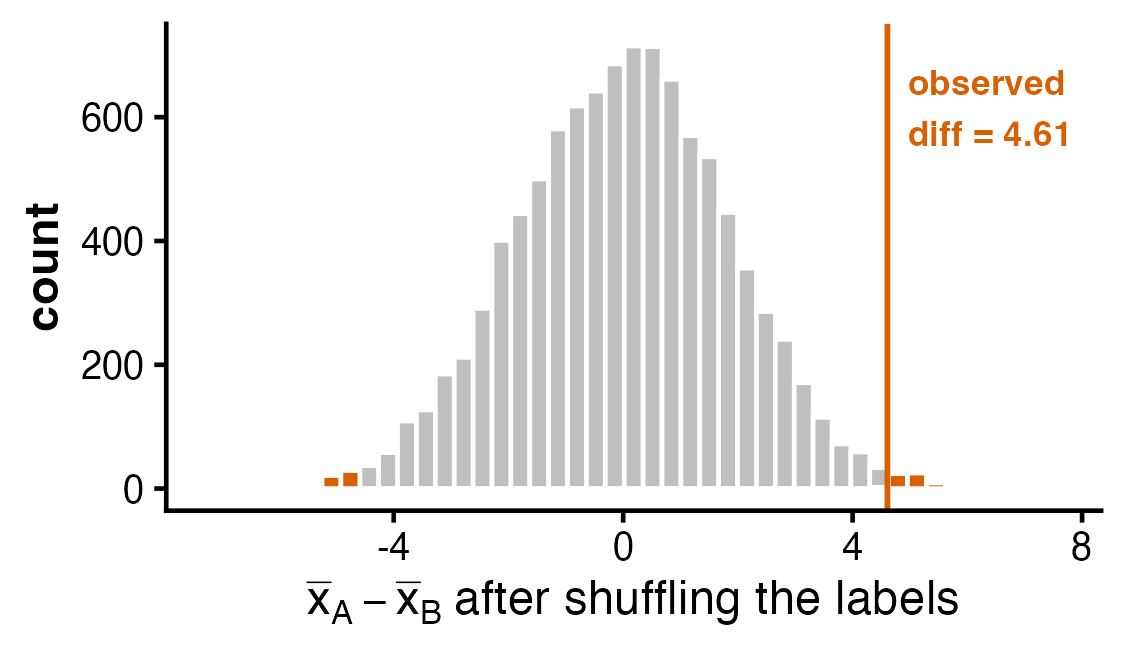
\includegraphics[width=\textwidth]{null-dist-permutation.png}
\end{center}
\column{0.48\textwidth}
\begin{center}
{\scriptsize Lecture 9: bootstrap resamples}\\[0.2em]
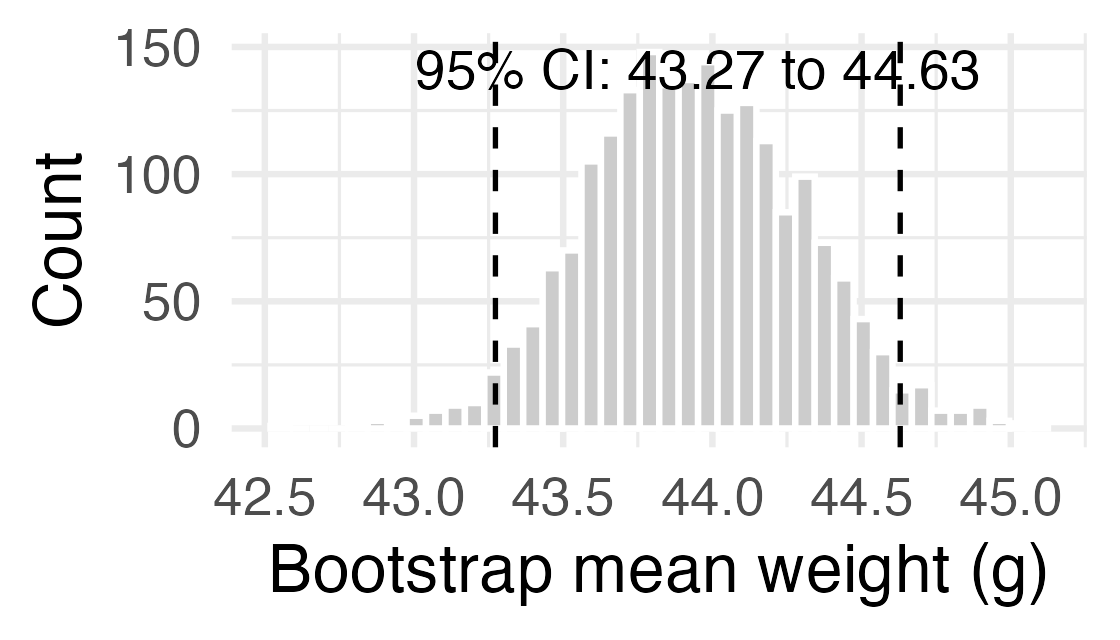
\includegraphics[width=\textwidth]{dm1999_boot_mean.png}
\end{center}
\end{columns}

\vspace{0.2em}
{\small Different data, different question, different simulation --- and neither was \emph{designed} to be bell-shaped. One shuffled quiz scores; the other resampled a lumpy, left-skewed pile of rat weights.}

\vspace{0.1em}
\dq{Coincidence? Or is something forcing this shape?}

\end{frame}

%%%%%%%%%%%%%%%%%%%%%%%%%%%%%%%%%%%%%%%%%%%%%%%%%%%%%%%%%%%%%%%%%%%%%%%%
\begin{frame}
\frametitle{The central limit theorem}

\keyidea[-- the CLT]{Take a sample of size $n$ from \emph{any} population with mean $\mu$ and standard deviation $\sigma$. Once $n$ is large enough, the sampling distribution of $\bar{x}$ is approximately normal, \textbf{whatever the population looks like}.}

\vspace{0.2em}
\formula{Standard errors from the CLT}{
\[
\bar{x} \;\approx\; N\!\left(\mu,\; \mathrm{SE}(\bar{x})\right),
\qquad
\mathrm{SE}(\bar{x}) \;=\; \frac{\sigma}{\sqrt{n}} \;\approx\; \frac{s}{\sqrt{n}} .
\]
A proportion is just the mean of a column of 0s and 1s, so the same theorem covers it: $\;\mathrm{SE}(\hat{p}) = \sqrt{p(1-p)/n}$.}

\vspace{-0.2em}
{\small Center, spread \emph{and} shape, with nothing resampled.}

\end{frame}

%%%%%%%%%%%%%%%%%%%%%%%%%%%%%%%%%%%%%%%%%%%%%%%%%%%%%%%%%%%%%%%%%%%%%%%%
\begin{frame}
\frametitle{``No matter what the population looks like''}

\begin{center}
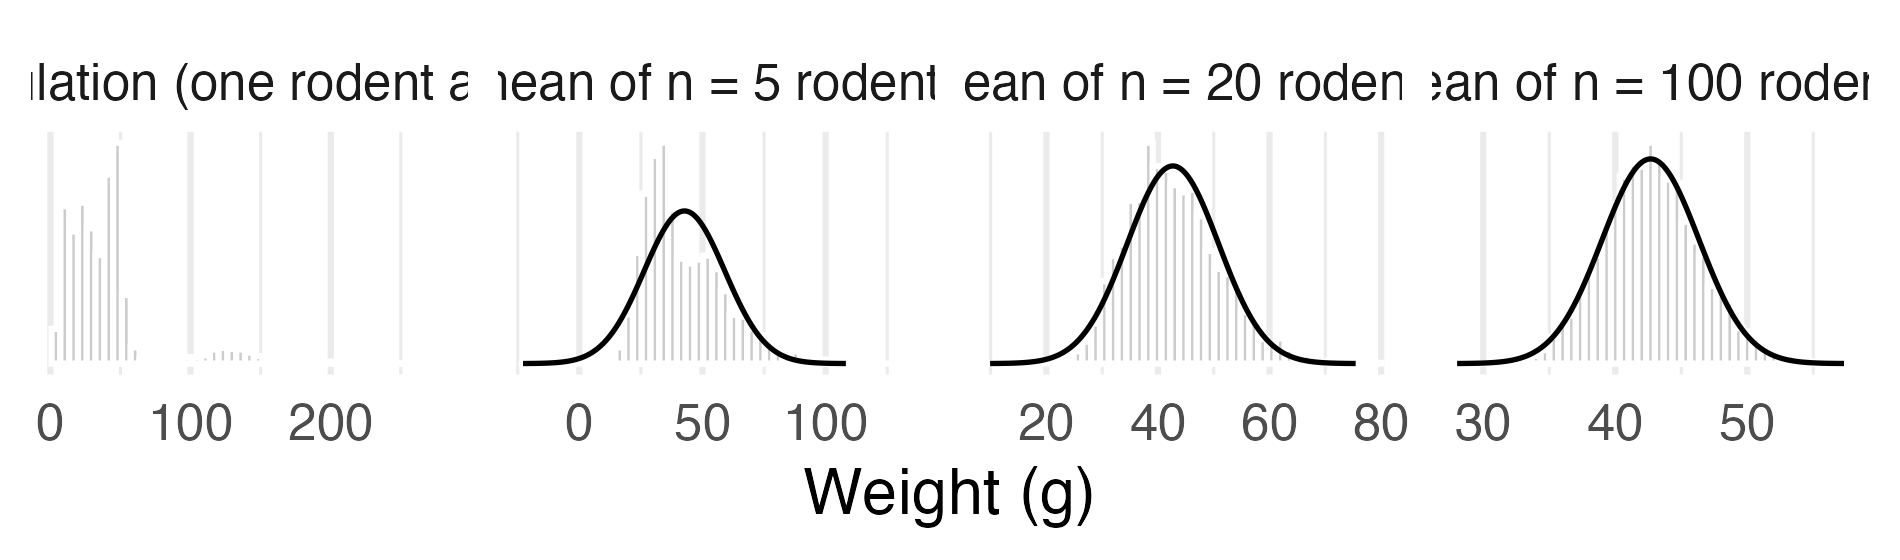
\includegraphics[width=0.99\textwidth]{clt_emerges.png}
\end{center}

\vspace{-0.4em}
{\small The population (left) is every rodent trapped at the site: several species pooled, wildly right-skewed, from $4$ g to $280$ g. Nothing normal about it. Yet the mean of $100$ of them lands almost exactly on the curve the CLT predicts --- a curve drawn from $\mu$ and $\sigma$ alone, \emph{without looking at the histogram}.}

\end{frame}

%%%%%%%%%%%%%%%%%%%%%%%%%%%%%%%%%%%%%%%%%%%%%%%%%%%%%%%%%%%%%%%%%%%%%%%%
\begin{frame}
\frametitle{The formula reproduces last lecture's bootstrap}

\vspace{-0.2em}
\begin{center}
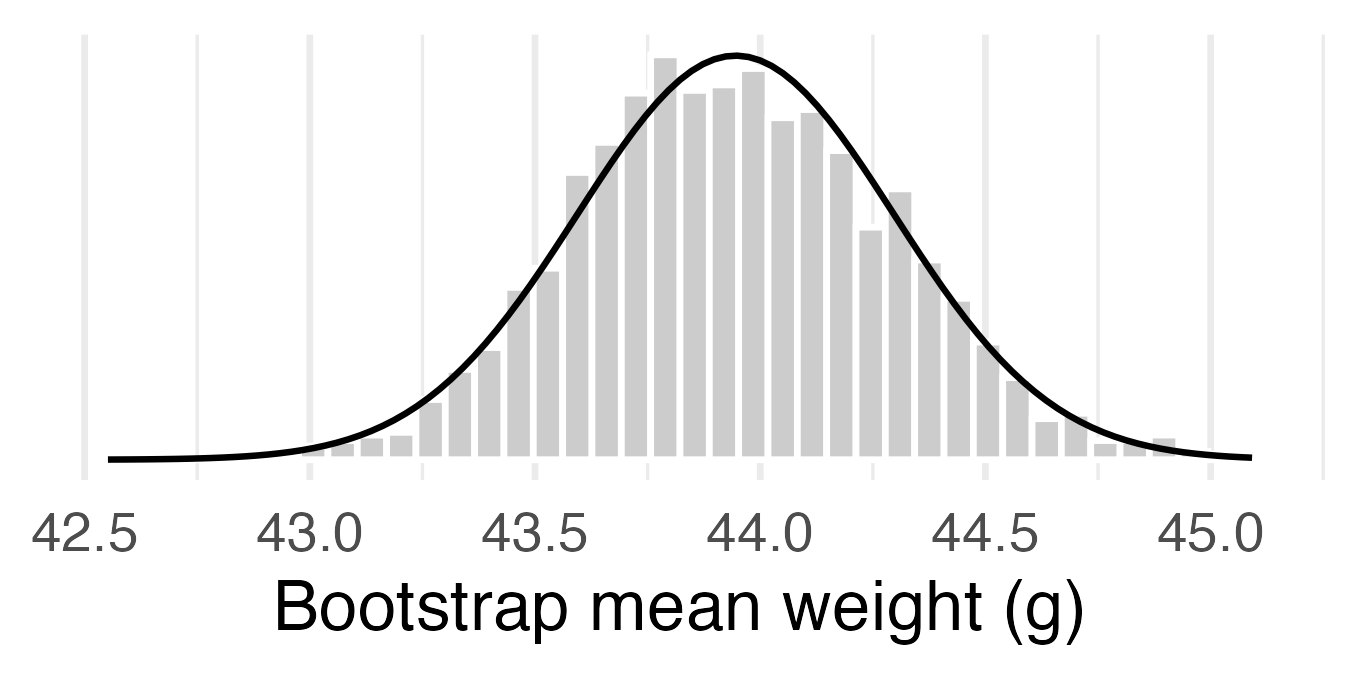
\includegraphics[width=0.68\textwidth]{clt_vs_bootstrap.png}
\end{center}

\vspace{-0.5em}
\keyidea[-- the point of today]{Two roads that share nothing: one resampled the data $2{,}000$ times, the other simply divided $s$ by $\sqrt{n}$. They land within $1\%$ of each other --- $0.355$ against $\hl{0.352}$.}

\end{frame}

%%%%%%%%%%%%%%%%%%%%%%%%%%%%%%%%%%%%%%%%%%%%%%%%%%%%%%%%%%%%%%%%%%%%%%%%
\begin{frame}
\frametitle{When does the CLT apply?}

\begin{itemize}
\item \hl{Independence.} The observations must be independent --- a random sample, or a randomised experiment.
\item \hl{Sample size.} ``Large enough'' depends on the population: the more skewed it is, the larger $n$ has to be. Look again at the $n=5$ panel --- the CLT curve did \emph{not} fit.
\item \hl{For proportions,} the usual rule is $np \ge 10$ and $n(1-p) \ge 10$: enough successes \emph{and} enough failures.
\end{itemize}

\vspace{0.3em}
\caution{The CLT is an \emph{approximation} that improves with $n$ --- not a licence to use a normal curve on any sample. With $n = 5$, or a statistic that is not a mean, it simply does not hold. That is exactly when we go back to bootstrapping.}

\end{frame}

%%%%%%%%%%%%%%%%%%%%%%%%%%%%%%%%%%%%%%%%%%%%%%%%%%%%%%%%%%%%%%%%%%%%%%%%
\section{P-values and intervals from a formula}
%%%%%%%%%%%%%%%%%%%%%%%%%%%%%%%%%%%%%%%%%%%%%%%%%%%%%%%%%%%%%%%%%%%%%%%%
\begin{frame}
\frametitle{The confidence interval, without resampling}

Write $\theta$ for whatever parameter we are after ($\mu$, $p$, $\mu_1 - \mu_2$, \ldots) and $\hat{\theta}$ for the estimate we computed from the sample. If its sampling distribution is normal, the middle $95\%$ sits within $1.96$ standard errors of the center:

\vspace{0.1em}
\formula{Confidence interval from the CLT}{
\[
\hat{\theta} \;\pm\; z^{*} \times \mathrm{SE},
\qquad z^{*} = 1.96 \ (95\%), \; 1.645 \ (90\%), \; 2.576 \ (99\%) .
\]}

\vspace{0.2em}
\hl{So that is where Lecture 9's ``$\pm\,2\,\mathrm{SE}$'' came from.} It was this formula all along, with $1.96$ rounded to $2$ --- and with $\mathrm{SE}$ estimated by resampling instead of computed.

\end{frame}

%%%%%%%%%%%%%%%%%%%%%%%%%%%%%%%%%%%%%%%%%%%%%%%%%%%%%%%%%%%%%%%%%%%%%%%%
\begin{frame}
\frametitle{Three roads to the same interval}

A 95\% confidence interval for the mean weight of a kangaroo rat, $n = 348$:

\vspace{0.2em}
{\small
\begin{center}
\begin{tabular}{lll}
\toprule
Method & Where the SE came from & 95\% CI (g) \\
\midrule
Bootstrap percentile & 2000 resamples & $[43.27,\; 44.63]$ \\
Bootstrap $\pm 2\,\mathrm{SE}$ & 2000 resamples & $[43.24,\; 44.65]$ \\
\hl{CLT formula} & $s/\sqrt{n} = 6.56/\sqrt{348}$ & $\hl{[43.26,\; 44.63]}$ \\
\bottomrule
\end{tabular}
\end{center}}

\vspace{0.3em}
The third row took no simulation at all --- and one of the $2{,}000$-resample rows agrees with it to the last decimal place shown.

\end{frame}

%%%%%%%%%%%%%%%%%%%%%%%%%%%%%%%%%%%%%%%%%%%%%%%%%%%%%%%%%%%%%%%%%%%%%%%%
\begin{frame}[fragile]
\frametitle{The $z$-test: Lecture 8's office hours, redone}

$29$ of $40$ students prefer online office hours. $H_0: p = 0.5$.

\vspace{-0.2em}
\begin{lstlisting}[language=R, basicstyle=\ttfamily\scriptsize]
phat <- 29/40                     # 0.725
se0  <- sqrt(0.5 * 0.5 / 40)      # SE *under H0* = 0.0791
z    <- (phat - 0.5) / se0        # 2.85
2 * pnorm(-abs(z))                #> 0.0044
\end{lstlisting}

\vspace{-0.2em}
\formula{The $z$-test}{
\[
z \;=\; \frac{\hat{\theta} - \theta_0}{\mathrm{SE}}, \qquad
p\text{-value} \;=\; 2\,P(Z > |z|) \quad\text{(two-sided)} .
\]}

\vspace{-0.1em}
{\small Note $\mathrm{SE}$ is computed \emph{under $H_0$}: we use $p_0 = 0.5$, not $\hat{p}$ --- the null world is the one we are testing.}

\end{frame}

%%%%%%%%%%%%%%%%%%%%%%%%%%%%%%%%%%%%%%%%%%%%%%%%%%%%%%%%%%%%%%%%%%%%%%%%
\begin{frame}
\frametitle{Three methods, one conclusion}

{\small
\begin{center}
\begin{tabular}{lll}
\toprule
Method & p-value & Cost \\
\midrule
Randomization (Lecture 8) & $0.005$ & $10{,}000$ simulations \\
$z$-test (today) & $0.0044$ & one line, but an approximation \\
\hl{Exact binomial} & $\hl{0.0064}$ & one line, and exact \\
\bottomrule
\end{tabular}
\end{center}}

\vspace{0.3em}
Look back at Lecture 8's table of ``how many simulations is enough''. Its last column was headed \textbf{exact}, and read $0.0064$ --- we never said where that number came from.

\vspace{0.2em}
\keyidea[-- the loop closes]{It came from the binomial. Simulation was \emph{approximating} a number the formula gives outright.}

\end{frame}

%%%%%%%%%%%%%%%%%%%%%%%%%%%%%%%%%%%%%%%%%%%%%%%%%%%%%%%%%%%%%%%%%%%%%%%%
\section{When sigma is unknown: the $t$ distribution}
%%%%%%%%%%%%%%%%%%%%%%%%%%%%%%%%%%%%%%%%%%%%%%%%%%%%%%%%%%%%%%%%%%%%%%%%
\begin{frame}
\frametitle{We used $\sigma$. We only have $s$.}

The CLT says $\bar{x} \approx N(\mu, \sigma/\sqrt{n})$ --- but $\sigma$ is a \emph{population} quantity. We never have it. We plug in the sample $s$ instead.

\vspace{0.4em}
\keyidea[-- what that costs]{Replacing $\sigma$ by an \emph{estimate} adds a second source of uncertainty on top of the sampling variability. The result is no longer normal: it has \textbf{heavier tails}. That distribution is the \hl{$t$ distribution}, with $n-1$ degrees of freedom.}

\vspace{0.4em}
Everything else is unchanged. The interval is still $\hat{\theta} \pm (\text{critical value}) \times \mathrm{SE}$ --- we just take the critical value from $t_{n-1}$ rather than from the normal.

\end{frame}

%%%%%%%%%%%%%%%%%%%%%%%%%%%%%%%%%%%%%%%%%%%%%%%%%%%%%%%%%%%%%%%%%%%%%%%%
\begin{frame}
\frametitle{How much heavier?}

\vspace{-0.2em}
\begin{center}
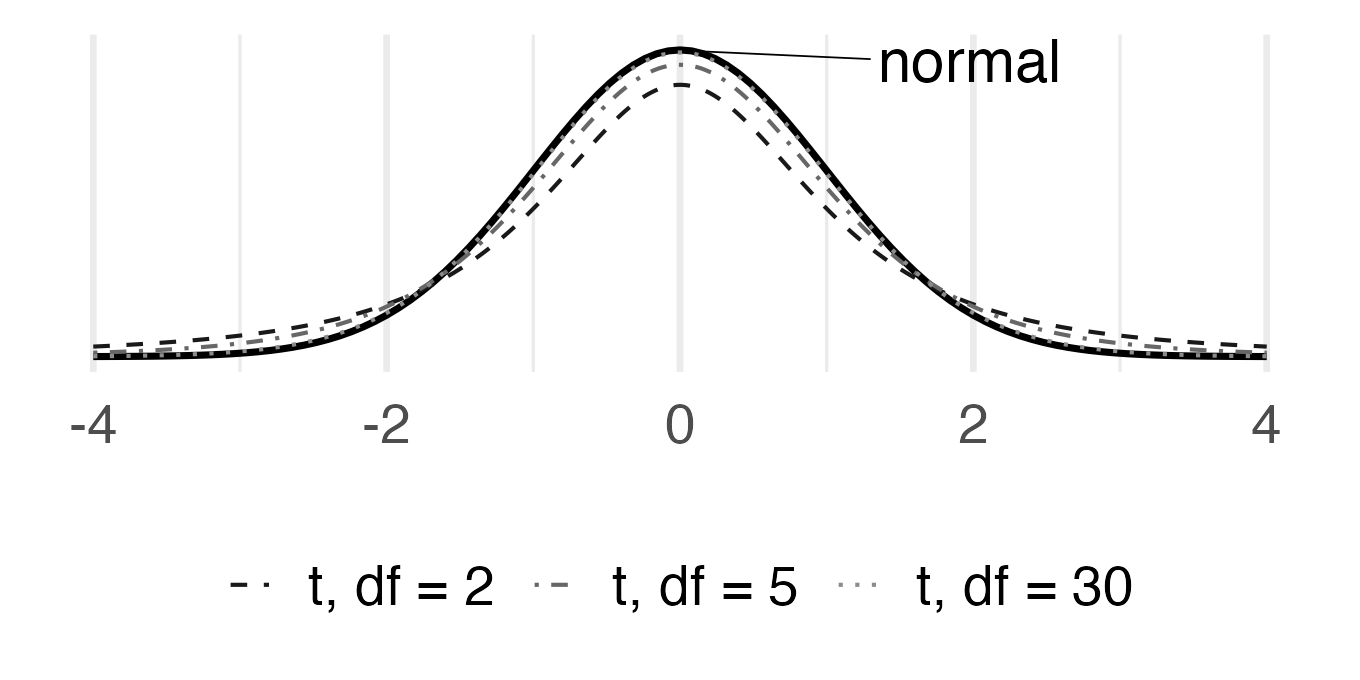
\includegraphics[width=0.62\textwidth]{t_vs_normal.png}
\end{center}

\vspace{-0.5em}
{\footnotesize
\begin{center}
\begin{tabular}{lccccc}
\toprule
& $df=2$ & $df=5$ & $df=30$ & $df=347$ & normal \\
\midrule
95\% critical value & 4.303 & 2.571 & 2.042 & \hl{1.967} & \hl{1.960} \\
\bottomrule
\end{tabular}
\end{center}}

\vspace{-0.2em}
{\small Strictly, the earlier interval should have used $1.967$, not $1.960$. With $n = 348$ that moves it by less than a thousandth of a gram. With $n = 5$ it would more than double it.}

\end{frame}

%%%%%%%%%%%%%%%%%%%%%%%%%%%%%%%%%%%%%%%%%%%%%%%%%%%%%%%%%%%%%%%%%%%%%%%%
\begin{frame}
\frametitle{So when does it matter?}

\begin{itemize}
\item \hl{Large $n$:} $t$ and $z$ are practically the same. Use either.
\item \hl{Small $n$:} the $t$ interval is genuinely wider --- and the honest one, because with a handful of observations $s$ is a poor estimate of $\sigma$.
\item In practice: \textbf{if you estimated the standard deviation from the data, use $t$.} R's \texttt{t.test()} does this by default.
\end{itemize}

\vspace{0.4em}
\keyidea[-- coming back in Lecture 13]{The same $t$ turns up in regression. To test whether a slope is zero we will compute $T = \hat{\beta}_1/\mathrm{SE}(\hat{\beta}_1)$ and compare it against $t_{n-2}$ --- the same idea, with two coefficients estimated instead of one.}

\end{frame}

%%%%%%%%%%%%%%%%%%%%%%%%%%%%%%%%%%%%%%%%%%%%%%%%%%%%%%%%%%%%%%%%%%%%%%%%
\section{Two samples and paired data}
%%%%%%%%%%%%%%%%%%%%%%%%%%%%%%%%%%%%%%%%%%%%%%%%%%%%%%%%%%%%%%%%%%%%%%%%
\begin{frame}
\frametitle{Comparing two independent groups}

The statistic is $\bar{x}_1 - \bar{x}_2$. It has its own standard error, and the CLT applies to it too.

\vspace{0.2em}
\formula{Standard error of a difference}{
\[
\mathrm{SE}(\bar{x}_1 - \bar{x}_2) \;=\; \sqrt{\frac{s_1^2}{n_1} + \frac{s_2^2}{n_2}} .
\]}

\vspace{0.2em}
{\small Variances add; standard errors do not. Note what this says: comparing two groups is \emph{harder} than estimating one, because both groups contribute noise.}

\vspace{0.2em}
The interval and the test are then exactly as before: $(\bar{x}_1 - \bar{x}_2) \pm t^{*}\,\mathrm{SE}$, and $t = (\bar{x}_1 - \bar{x}_2)/\mathrm{SE}$.

\end{frame}

%%%%%%%%%%%%%%%%%%%%%%%%%%%%%%%%%%%%%%%%%%%%%%%%%%%%%%%%%%%%%%%%%%%%%%%%
\begin{frame}
\frametitle{Do male and female kangaroo rats differ in weight?}

\vspace{-0.2em}
\begin{center}
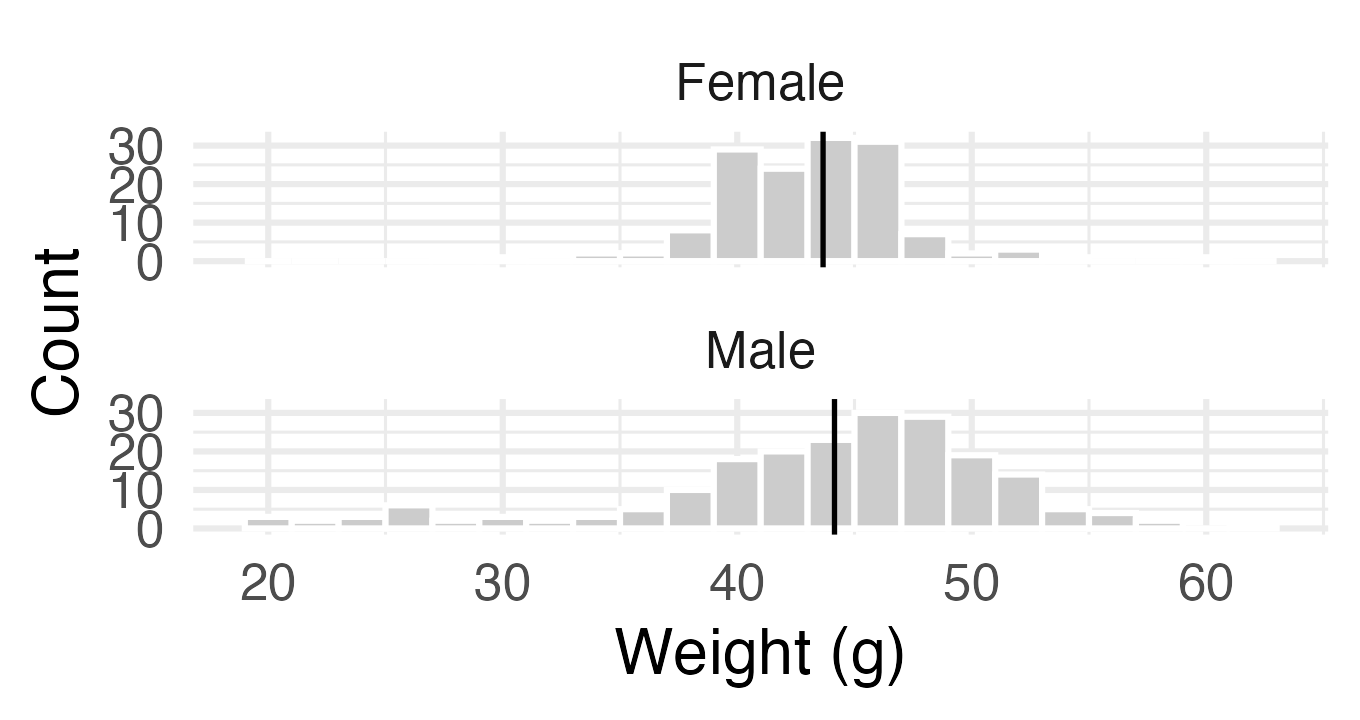
\includegraphics[width=0.60\textwidth]{two_sample_sex.png}
\end{center}

\vspace{-0.5em}
{\small
Males average $44.15$ g ($n=204$), females $43.66$ g ($n=144$): a difference of $0.49$ g with $\mathrm{SE} = 0.65$.
\[
t = \frac{0.49}{0.65} = 0.75 \;\;(df \approx 319), \qquad p = 0.45, \qquad \text{95\% CI} = [-0.78,\; 1.76] .
\]
The interval contains zero. \hl{No evidence of a difference} --- the gap between the groups is swamped by the variation within them.}

\end{frame}

%%%%%%%%%%%%%%%%%%%%%%%%%%%%%%%%%%%%%%%%%%%%%%%%%%%%%%%%%%%%%%%%%%%%%%%%
\begin{frame}
\frametitle{Paired data is not two samples}

A bookshop and Amazon both stock the same $73$ textbooks. We have two prices for \emph{each book}.

\vspace{0.4em}
\keyidea[-- the move]{When every observation in one group has a natural partner in the other, the data are \hl{paired}. Take the difference \emph{within each pair} --- and a two-sample problem collapses into a \textbf{one-sample} problem about the mean difference.}

\vspace{0.4em}
Why bother? Because a $\$200$ physics text and a $\$15$ paperback differ from each other far more than either differs between the two shops. Pairing subtracts that irrelevant variation away.

\end{frame}

%%%%%%%%%%%%%%%%%%%%%%%%%%%%%%%%%%%%%%%%%%%%%%%%%%%%%%%%%%%%%%%%%%%%%%%%
\begin{frame}
\frametitle{The same data, paired or not}

\vspace{-0.3em}
\begin{center}
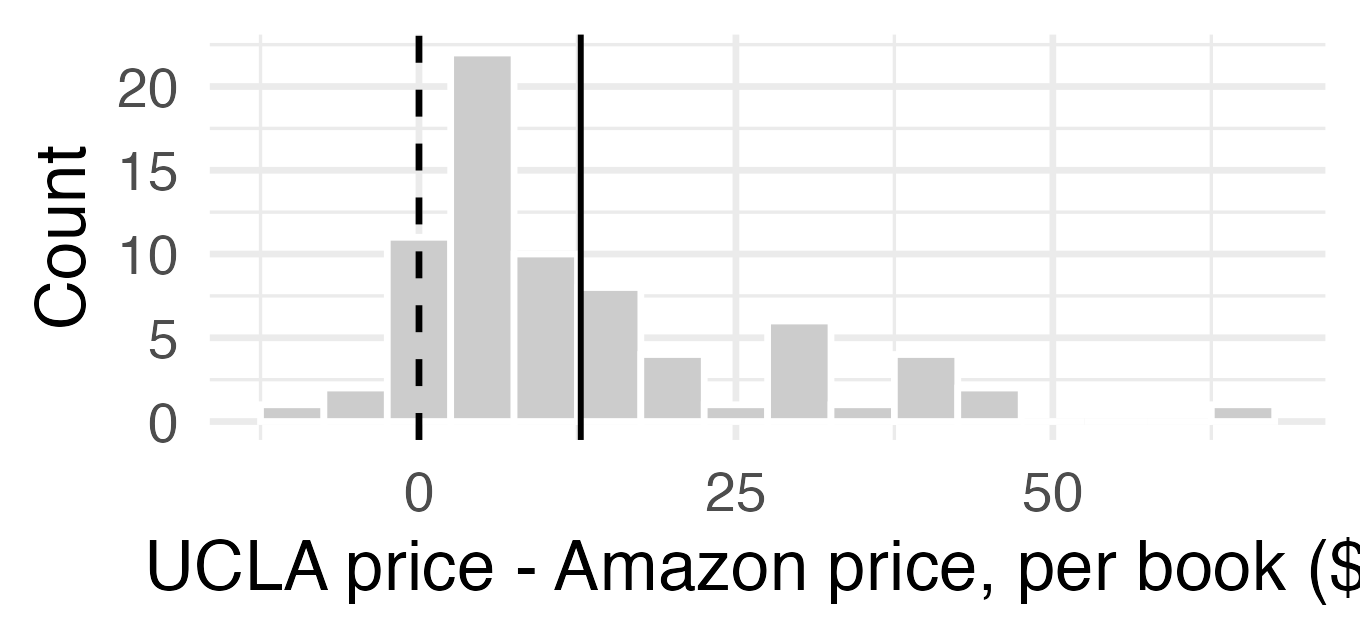
\includegraphics[width=0.42\textwidth]{paired_textbooks.png}
\end{center}

\vspace{-0.5em}
{\footnotesize
\begin{center}
\begin{tabular}{lll}
\toprule
Analysis & p-value & 95\% CI for the difference \\
\midrule
\hl{Paired} (correct) & $7 \times 10^{-11}$ & $[\$9.44,\; \$16.09]$ \\
Two independent samples & $0.16$ & --- \\
\bottomrule
\end{tabular}
\end{center}}

\vspace{-0.2em}
\caution{Same $73$ books, same two prices. Ignore the pairing and the \$12.76 difference vanishes into the noise --- \emph{opposite conclusions from identical data.}}

\end{frame}

%%%%%%%%%%%%%%%%%%%%%%%%%%%%%%%%%%%%%%%%%%%%%%%%%%%%%%%%%%%%%%%%%%%%%%%%
\begin{frame}
\frametitle{Activity: paired or two-sample?}

\app{
For each study, say whether the data are paired or two independent samples --- and what the statistic would be.

\begin{enumerate}
\item Blood pressure of $30$ patients, measured before and after a drug.
\item Weights of the $204$ male and $144$ female rats we trapped.
\item Exam scores of two different discussion sections.
\item The same $50$ runners' times in April and in September.
\item Yields from $12$ farms, each split into a treated half and an untreated half.
\end{enumerate}}

\end{frame}

%%%%%%%%%%%%%%%%%%%%%%%%%%%%%%%%%%%%%%%%%%%%%%%%%%%%%%%%%%%%%%%%%%%%%%%%
\begin{frame}
\frametitle{Activity: paired or two-sample? --- solution}

\solnbox{\small \textbf{Paired:} (1) each patient is their own control; (4) each runner appears twice; (5) the two halves of a farm share its soil and weather. In all three, compute the \emph{difference within each pair} and do a one-sample analysis of those differences. \textbf{Two independent samples:} (2) and (3) --- no rat is both male and female, no student sits in both sections, so there is nothing to pair up. Use $\bar{x}_1 - \bar{x}_2$ with $\mathrm{SE} = \sqrt{s_1^2/n_1 + s_2^2/n_2}$.}

\vspace{0.4em}
The test to apply: \hl{can you draw a line between one observation in group A and exactly one in group B?} If yes, pair them. If the two groups even have different sizes, they cannot be paired.

\end{frame}

%%%%%%%%%%%%%%%%%%%%%%%%%%%%%%%%%%%%%%%%%%%%%%%%%%%%%%%%%%%%%%%%%%%%%%%%
\section{Formula versus simulation}
%%%%%%%%%%%%%%%%%%%%%%%%%%%%%%%%%%%%%%%%%%%%%%%%%%%%%%%%%%%%%%%%%%%%%%%%
\begin{frame}
\frametitle{Three ways to get a sampling distribution --- completed}

{\scriptsize
\begin{center}
\setlength{\tabcolsep}{4pt}
\begin{tabular}{p{0.13\textwidth}p{0.22\textwidth}p{0.22\textwidth}p{0.27\textwidth}}
\toprule
& \textbf{Randomization} \newline (Lecture 8) & \textbf{Bootstrap} \newline (Lecture 9) & \textbf{Mathematical model} \newline (today) \\
\midrule
Starts from & a null hypothesis & the observed sample & a probability model \\
Builds & a null distribution & a sampling distribution & a \emph{formula} for it \\
Gives you & a p-value & a confidence interval & both, instantly \\
Needs & a computer & a computer & the conditions to hold \\
Works for & any statistic & any statistic & means, proportions, differences \\
\bottomrule
\end{tabular}
\end{center}}

\vspace{0.2em}
{\small The three agree whenever they are all valid --- we have now checked that twice, on the rats and on the office hours.}

\end{frame}

%%%%%%%%%%%%%%%%%%%%%%%%%%%%%%%%%%%%%%%%%%%%%%%%%%%%%%%%%%%%%%%%%%%%%%%%
\begin{frame}
\frametitle{So which one should I use?}

\begin{itemize}
\item \hl{A formula exists and its conditions hold} $\Rightarrow$ use it. Exact or nearly so, instant, and free of simulation noise.
\item \hl{An unusual statistic} --- a median, a 90th percentile, a maximum $\Rightarrow$ no formula exists. Bootstrap it.
\item \hl{A null you can simulate but not solve} $\Rightarrow$ randomization.
\end{itemize}

\vspace{0.4em}
\caution{These are two routes to the \emph{same} sampling distribution --- not ``the truth'' and ``an approximation to it''. Each one fails in situations where the other works.}

\end{frame}

%%%%%%%%%%%%%%%%%%%%%%%%%%%%%%%%%%%%%%%%%%%%%%%%%%%%%%%%%%%%%%%%%%%%%%%%
\begin{frame}
\frametitle{And when $n$ is small?}

Neither road is free.

\begin{itemize}
\item The \hl{CLT has not kicked in}, so a $t$ interval is valid only if the \emph{population itself} is roughly normal --- an assumption you now have to argue for, not one the theorem hands you.
\item And \hl{the bootstrap cannot rescue a tiny sample} either: with $n=5$ every resample reuses the same five numbers (Lecture 9).
\end{itemize}

\vspace{0.4em}
\keyidea[-- the honest answer]{With $n = 6$, no arithmetic manufactures information the data do not contain. The right move is to say so --- and, if it matters, to go and catch more rats.}

\end{frame}

%%%%%%%%%%%%%%%%%%%%%%%%%%%%%%%%%%%%%%%%%%%%%%%%%%%%%%%%%%%%%%%%%%%%%%%%
\section{Wrap-up}
%%%%%%%%%%%%%%%%%%%%%%%%%%%%%%%%%%%%%%%%%%%%%%%%%%%%%%%%%%%%%%%%%%%%%%%%
\begin{frame}
\frametitle{Summary}

\begin{itemize}
\item Some sampling distributions are known \emph{exactly}: the \hl{binomial} for counts of successes.
\item The \hl{central limit theorem}: for large enough $n$, $\bar{x} \approx N(\mu,\, \sigma/\sqrt{n})$ whatever the population looks like. This is why our simulated distributions kept coming out bell-shaped.
\item From it: $\;\hat{\theta} \pm z^{*}\mathrm{SE}\;$ for intervals, $\;z = (\hat{\theta}-\theta_0)/\mathrm{SE}\;$ for tests.
\item $\sigma$ is never known. Using $s$ instead gives the \hl{$t$ distribution}: heavier tails, same recipe.
\item Two groups: $\mathrm{SE} = \sqrt{s_1^2/n_1 + s_2^2/n_2}$. \hl{Paired data is not two samples}: difference the pairs first.
\item Formulas are instant but conditional; simulation is general but needs a computer. \emph{Neither} rescues a sample that is too small.
\end{itemize}

\end{frame}

%%%%%%%%%%%%%%%%%%%%%%%%%%%%%%%%%%%%%%%%%%%%%%%%%%%%%%%%%%%%%%%%%%%%%%%%
\begin{frame}
\frametitle{Coming up next}

\hl{Next class, testing for independence:} what if both variables are \emph{categorical}? Is a student's class year related to whether they prefer online office hours?

\begin{itemize}
\item \hl{two-way tables} and what ``independent'' would predict for their cells;
\item the same two roads again: shuffle the labels, or use a mathematical model;
\item and the model, this time, is the \hl{chi-square distribution}.
\end{itemize}

\vspace{0.3em}
\emph{To think about:} three ways to build a sampling distribution keep agreeing. What would it mean if they disagreed?

\end{frame}

%%%%%%%%%%%%%%%%%%%%%%%%%%%%%%%%%%%%%%%%%%%%%%%%%%%%%%%%%%%%%%%%%%%%%%%%

%%%%%%%%%%%%%%%%%%%%%%%%%%%%%%%%%%%%
% End document
%%%%%%%%%%%%%%%%%%%%%%%%%%%%%%%%%%%%

\end{document}
